\subsubsection{Bokonongo-Gruppe}\label{sec:BOG-Gr}

An fünf Fundstellen entlang des unteren \mbox{Sangha} sowie an zweien am Kongo (Abb.~\ref{fig:BOG_Verbreitung}) wurden bei Surveys sehr charakteristische keramische Formen gefunden, die mit einer Ausnahme\footnote{Lediglich in Sosolo an der Mündung des \mbox{Sangha} (Fpl.~241) wurden zehn GE gefunden, die der Bokonogo-Gruppe zugeweisen werden können.} fast ausschließlich als Einzelfunde an den jeweiligen Plätzen auftraten. Die nach dem eponymen Fundort Bokono\-ngo am mittleren \mbox{Sangha} (Fpl.~250) benannte Stilgruppe zeichnet sich durch eine spezifische Ausgestaltung des Gefäßrandes bei einer der beiden beobachteten Gefäßformen aus: kurze, konvex ausbiegende Ränder (B3.1), die häufig in einem geraden, zylindrischen Mündungsabschluss enden (Abb.~\ref{fig:BOG-Typen}.1--4). Zudem umfasst das Formenspektrum der Bokonongo-Gruppe noch Schalen mit einbiegendem Rand (Abb.~\ref{fig:BOG-Typen}.5--9).

Insgesamt wurden 19~GE beobachtet, die der Stilgruppe zugerechnet werden können. Alle Stücke stammen aus Oberflächenabsammlungen, wodurch die mögliche Vergesellschaftung dieser mit anderen Formen sowie ihre chronologische Einordnung stark eingeschränkt ist. Eine ähnlich spezifische Ausprägung der Randgestaltung findet sich bislang nur in der als Oveng-Gruppe geführten, früheisenzeitlichen Keramik aus Gabun \parencites[615--618]{Clist.20042005}[134 Abb. 15]{GonzalesRuibal.2012}[217--299]{SanchezElipe.2015}[351--355]{SanchezElipe.2016}. Lose erinnert sie aber auch an einige Ränder des Pikunda-Munda-Stils (Abb.~\ref{fig:PIKMUN_TypVertreter}.3, 5; Taf.~50.7). Die Bokonongo-Gruppe setzt sich aus drei vollständigen oder hinreichend erhaltenen Gefäßen (Abb.~\ref{fig:BOG-Typen}.3--4; Taf.~54.1) sowie 16 großen Randfragmenten zusammen. In Anbetracht der spärlichen Datenlage kann die postulierte Zusammengehörigkeit der hier als Bokonongo-Stil systematisierten keramischen Formen lediglich als Provisorium angesehen werden.

\begin{figure*}[!tb]
	\centering
	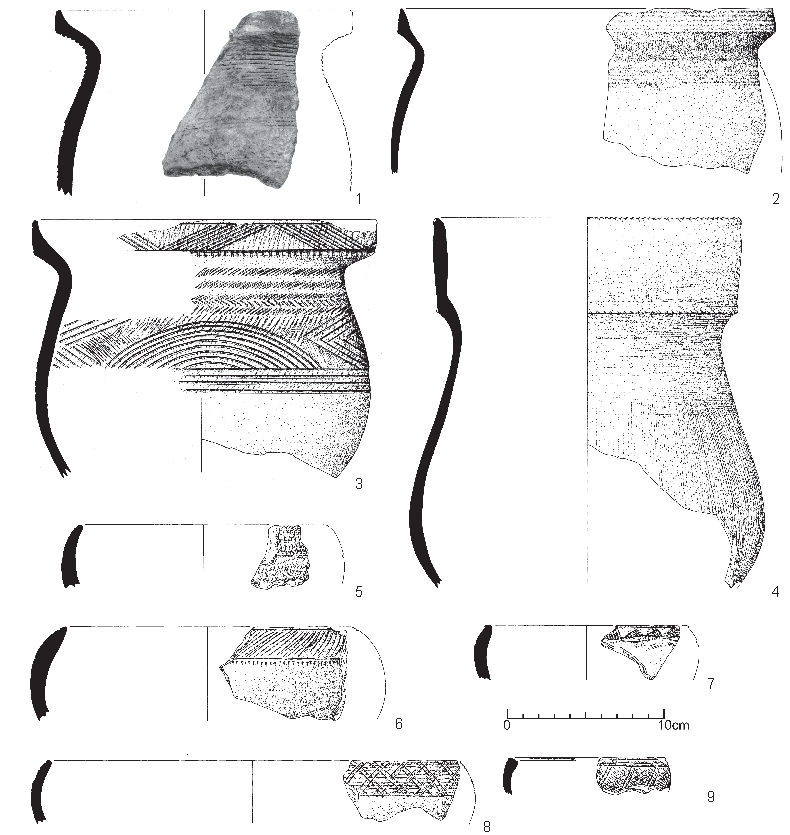
\includegraphics[width=\textwidth]{fig/BOG-Typen.pdf}
	\caption{Bokonongo-Gruppe: Typvertreter im nordwestlichen Kongobecken.\\1:~Taf.~40.3; 2:~Taf.~35.9; 3:~Taf.~40.8; 4:~Taf.~51.11; 5: Taf.~29.3; 6: Taf.~36.1; 7: Taf.~36.4; 8: Taf.~29.5; 9: Taf.~32.13.}
	\label{fig:BOG-Typen}
\end{figure*}

\begin{figure*}[p]
	\centering
	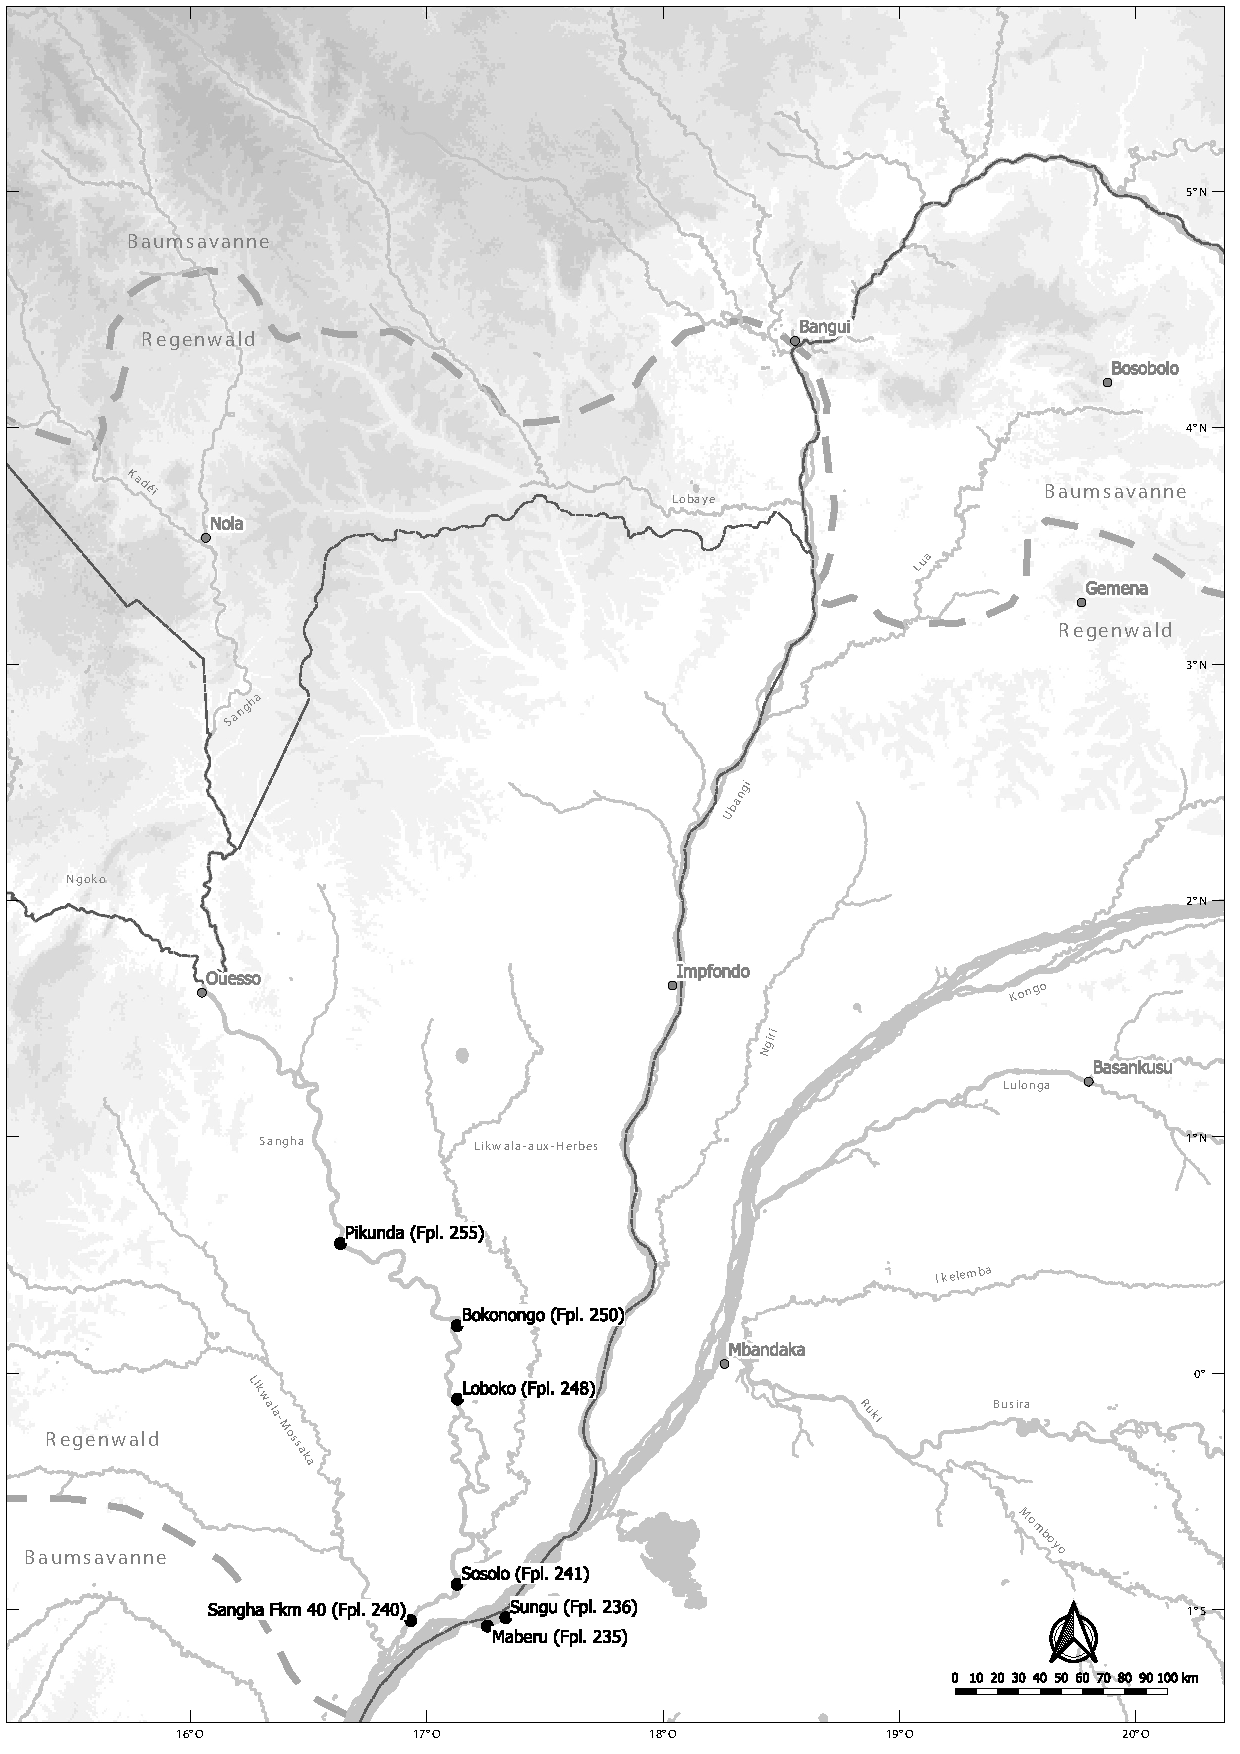
\includegraphics[width=\textwidth]{fig/BOG_Verbreitung.pdf}
	\caption{Bokonongo-Gruppe: Verbreitung.}
	% \caption{Bokonongo-Gruppe: Verbreitung (Kreise) und Verbreitung der Oveng-Keramik in Gabun \parencites[Dreiecke, nach][615 Fig. 7-58]{Clist.20042005}{GonzalezRuibal.2011}{GonzalesRuibal.2012}.}
	\label{fig:BOG_Verbreitung}
\end{figure*}

\paragraph{Technologische Merkmale}\hspace{-.5em}|\hspace{.5em}%
Zwei Drittel aller der Bokonongo-Gruppe zugerechneten GE zeigen einen Scherben, praktisch ohne nichtplastische Partikel des \textit{Fabrics} 1 und 2 (Tab.~\ref{tab:Fabrics_Bilder}). Diese GE enthalten durchweg weniger als 10\,\% nichtplastische Partikel, die den Größenklassen \textit{very fine} bis \textit{medium} zugerechnet werden können. Wurden nichtplastische Partikel in den Scherben beobachtet, handelte es sich ausnahmslos um heterogenen Quarzsand. Das andere Drittel weist Fragmente von zerstoßener Keramik im Scherben auf und kann den \textit{Fabrics} 8 und 9 zugerechnet werden. Vertreter des \textit{Fabrics} 8, das sich durch Schamott und andere nichtplastische Partikel auszeichnet, waren ebenso häufig vertreten, wie Stücke, die ausschließlich Schamott enthalten und dem \textit{Fabric} 9 zuzurechnen sind. Während knapp die Hälfte der GE (48\,\%) eine Färbung aufweist, die auf die Nutzung eines weißbrennenden Tones hindeuten, zeigen zwei GE die Nutzung rotbrennender Tone an. Die Oberflächen der Stücke sind durchweg glatt (76\,\%) oder nur leicht rau.

\paragraph{Formen}\hspace{-.5em}|\hspace{.5em}%
Eine der beiden Grundformen der Bokonongo-Gruppe und das bestimmende Charakteristikum für die Beschreibung der Stilgruppe sind Gefäße mit geschweifter Wandung und dem eingangs beschriebenen konvex ausbiegendem Rand mit zylindrischem Abschluss vom Typ B3.1 (Abb.~\ref{fig:BOG-Typen}.1--4). Diese machen knapp die Hälfte aller der Bokonongo-Gruppe zugeordneten GE aus. Die andere Hälfte bilden schalenförmige Gefäße mit konvexer Wandung und einbiegendem Rand vom Typ H2 (Abb.~\ref{fig:BOG-Typen}.5--9). Während die Gefäßbäuche durchweg konvex sind, liegen keine GE vor, bei der der Boden erhalten wäre.

\paragraph{Verzierungen}\hspace{-.5em}|\hspace{.5em}%
Die Verzierungen der Bokonongo-Keramik sind, ähnlich wie jene der Pikunda-Munda-Keramik, von Rillen (Tab.~\ref{tab:Verzierungselemente}: 01) und Riefen (Tab.~\ref{tab:Verzierungselemente}: 02) bestimmt. Diese machen zusammen 78\,\% aller beobachteten Verzierungselemente aus (Anlage~4\subref{fig:BOG_Verz}). Bestimmendes Verzierungselement sind horizontale Rillen, die sich vornehmlich auf der Außenseite des Randes finden (Tab.~\ref{tab:Verzierungselemente}: 02.1; 39\,\%), gefolgt von vertikalen Rillen (Tab.~\ref{tab:Verzierungselemente}:02.2; 12\,\%) und horizontalen Reihen feiner Eindrücke (Tab.~\ref{tab:Verzierungselemente}: 04.12; 8\,\%). Ebenso häufig lassen sich aus Ritzlinien gebildete Schachbrettmuster beobachten (Tab.~\ref{tab:Verzierungselemente}: 01.1--4; 10\,\%). Die Verzierung wird vornehmlich in Form horizontaler Bänder unterhalb des Randes sowie am oberhalb des maximalen Durchmessers gelegenen Teil des Gefäßbauches aufgebracht (Abb.~\ref{fig:BOG-Typen}.1--3, 5--9). In seltenen Fällen lassen sich auch flächige Verzierungen des gesamten Gefäßkörpers beobachten (Abb.~\ref{fig:BOG-Typen}.4). Basierend auf den der Bokonongo-Gruppe zugewiesenen Stücken scheint das Unterteil der Gefäße, bis auf wenige Ausnahmen (Abb.~\ref{fig:BOG-Typen}.4), konsequent frei von Verzierungen zu sein. Regelhaft lässt sich auch die Überlagerung von Verzierungselementen beobachten (Abb.~\ref{fig:BOG-Typen}.3, 8--9).

\paragraph{Datierung}\hspace{-.5em}|\hspace{.5em}%
Für das ausschließlich aus Oberflächenabsammlungen bekannte Material der Bokonongo-Grup"-pe sind keine absoluten Daten bekannt. Keines der Stücke stammt aus einem ergraben Kontext. Eine direkte Datierung der Funde oder auf Basis die Vergesellschaftung mit anderem Fundgut ist daher nicht möglich.

Auffällig ist die eingangs erwähnte Parallele der Randgestaltung der geschlossenen Gefäße (Abb.~\ref{fig:BOG-Typen}.1--4) zu Material der Oveng-Gruppe in Gabun. Die Verbreitung dieser Keramik beschränkt sich auf das direkte Umland von Libreville im Westen Gabuns (ebd. 615 Fig.~7-58) sowie die der Küste vorgelagerte, zu Äquatorialguinea gehörende Insel Corisco \parencite[217--221]{SanchezElipe.2015}.\footnote{Siehe auch \textsc{González-Ruibal} u.a. (2011; 2012).} Die genannten Ränder lassen sich lose mit  jener von \textcite[559 Abb.~7-18.D]{Clist.20042005} als Var. \enquote{D} bezeichneten Ausprägung der Oveng-Keramik in Verbindung bringen. Das Inventar eines Verhüttungsbefundes von der durch sein früheisenzeitliches Gräberfeld bekannten Insel Corisco \parencite[134 Abb.~15]{GonzalesRuibal.2012} weist deutliche Parallelen zur Keramik der Bokonongo-Gruppe auf. Auch der Fokus der Verzierung auf den Bereich ausschließlich unterhalb des Randes und die Verwendung von diagonalen Kammeindrücken sowie Winkel- und Fischgrätmustern lässt sich bei GE der Bokonongo-Gruppe beobachten (Abb.~\ref{fig:BOG-Typen}.3,6--7). Die Keramik der Oveng-Gruppe wird in das 2.~Jh. v.~Chr. bis 5.~Jh. n.~Chr. datiert \parencite[555 Fig.~7-14]{Clist.20042005}.\footnote{Dieser Zeitraum entspricht grob der vorliegenden Datierung für den Pikunda-Munda-Stil (Abb.~\ref{fig:PIKMUN_14C}).} Für die Keramik der Bokonongo-Gruppe wird vorläufig ein entsprechender Datierungsansatz vorgeschlagen.

\paragraph{Verbreitung}\hspace{-.5em}|\hspace{.5em}%
Keramik des Bokonongo-Stils findet sich ausschließlich am unteren \mbox{Sangha} sowie im Bereich der \mbox{Sangha}-Mündung (Abb.~\ref{fig:BOG_Verbreitung}). Während der Nachweis im Bereich der \mbox{Sangha}-Mündung mit vier eng beieinander liegenden Fundplätzen (Fpl.~235--236 und 240--241) noch als einigermaßen gut gelten kann, nimmt er weiter nach Norden, den \mbox{Sangha} flussauf, deutlich ab. Die nördlichste Fundstelle mit Keramik der Bokonongo-Gruppe ist Pikunda am mittleren \mbox{Sangha} (Fpl.~255).
